\documentclass[sigconf, review]{acmart}


\newcommand{\mat}[1]{\mathbf{#1}}
\renewcommand{\vec}[1]{\mathbf{#1}}

\begin{document}

\title{Simulating Hybrid Analog + RISC-V Systems for HPC Applications}

\author{Cameron Durbin}
\authornote{This work was conducted during an internship at Sandia National Laboratories}
\affiliation{%
  \institution{University of Oregon}
  \city{Eugene}
  \state{Oregon}
  \country{USA}
}
\email{cfd@uoregon.edu}

\author{Jacob Flores}
\affiliation{%
  \institution{Sandia National Laboratories}
  \city{Albuquerque}
  \state{New Mexico}
  \country{USA}
}
\email{jmflore@sandia.gov}

\author{Thomas Weatherly}
\authornotemark[1]
\affiliation{%
  \institution{Georgia Tech Research Institute}
  \city{Atlanta}
  \state{Georgia}
  \country{USA}
}
\email{Thomas.Weatherly@gtri.gatech.edu}

\author{Ben Feinberg}
\affiliation{%
  \institution{Sandia National Laboratories}
  \city{Albuquerque}
  \state{New Mexico}
  \country{USA}
}
\email{bfeinbe@sandia.gov}


\begin{abstract}

%\begin{itemize}
%    \item HPC is used across many domains.
%    \item To speedup HPC applications, accelerators are used.
%    \item Accelerators consume an enormous amount of power performing linear operations. 
%    \item Researchers are seeking new methods to compute at lower power.
%    \item Memristors have revived interest in analog crossbars, a low power semiconductor device for computing mvm.
%    \item Simulation offers insight into the performance and accuracy of novel architectures before being developed.
%    \item We assembled a simulation platform that enables researchers to experiment with analog architectures.
%    \item We wrote iterative linear solvers that are executed on our platform.
%    \item We run our programs through on out platform and provide performance metrics.
%\end{itemize}

As digital scaling trends have slowed over the past decade, there has been renewed interest in new computing paradigms such as analog.
Analog computing has the potential to provide performance and efficiency beyond what is achievable by digital systems; however, many challenges remain.
One such challenge is supporting complex applications using analog components that implement few computational kernels.
We consider on a class of hybrid analog + digital systems where analog accelerators are used as tightly integrated coprocessors within each core.
The RISC-V ISA simplifies the design of hybrid systems, providing a mature software stack for the digital components allowing system designers to focus on the analog-specific aspects of the architecture and software.
To investigate the viability of these architectures for high performance computing we evaluate two iterative linear solvers using hybrid analog + RISC-V processors using the Structural Simulation Toolkit.
% TODO Results sentence. 

% High-Performance Computing (HPC) is vital across a wide range of scientific and engineering domains.
% Modern systems achieve their performance gains through specialized hardware accelerators, but this often comes at the cost of substantial power draw, particularly for dense operations such as matrix-vector multiplications (MVMs).
% As energy efficiency becomes an increasingly critical constraint, researchers are exploring new hardware paradigms to compute MVMs at reduced energy costs.
% One promising direction is the use of analog crossbars-resistive memory arrays that naturally perform MVMs using Ohm's law.

% To investigate the viability of analog-digital hybrid architectures in HPC, we extended SST's RISC-V CPU model to support a RoCC-connected analog coprocessor.
% This platform enables exploration of realistic hardware behaviors, software interfaces, and execution patterns in an analog-digital hybrid environment.
% We demonstrate the platform's capability by running iterative linear solvers and reporting performance metrics that highlight trade-offs between accuracy, latency, and analog complexity.
% Our results offer early insight into the opportunities and challenges of integrating analog acceleration into future HPC architectures.

\end{abstract}

\keywords{RISC-V, High-Performance Computing, Emerging Memories}

\maketitle
\section{Introduction}

%\begin{itemize}
%    \item Data centers consume an enormous amount of power.
%    \item Power consumption is expected to double or triple by 2028.
%    \item Memristors have revived interest in crossbars mvm, a low power solution.
%    \item To implement crossbar mvms, hardware/software co-design must efficient be done.
%    \item Simulation is a powerful technique to build architecture prototypes.
%    \item We build a simulation platform that enables crossbar simulation capable of handling HPC loads.
%    \item There has been no work done in this field yet - open simulation stack
%    \item We contribute a full evaluation architecture + performance on ILS (CG)
%    \item The roadmap is to continue to build infrastructure surrounding it
%\end{itemize}

With the end of Dennard Scaling, the current technology trajectory for computer systems is toward higher power consumption for higher performance.
This trend, which applies from small embedded processors up to the largest high-performance computing and data centers, means that increasing problem scale or complexity requires an increasing system power budget.
To meet this concern, new technology paradigms, which do not rely on conventional digital technology, have become a major research interest with several showing potential for orders-of-magnitude improvements in energy efficiency at the operation level.
Analog linear algebra acceleration is one such paradigm, taking advantage of the ability of analog circuits to encode various computations. 
Although not a new idea, developments over the past decade in resistive memory technologies provide dense, programmable, and CMOS-compatible memories, enabling high programmability and integration scale for these analog accelerators.
Using these technologies, recent analog matrix-vector multiplication (MVM) prototypes have demonstrated greater-than-digital energy efficiency in systems with millions of individual resistive memories~\cite{ambrogio-energy-2023}.

A key challenge for the use of analog accelerators is how to effectively integrate them with conventional digital processing.
Even if analog components are responsible for the vast majority of the operations, digital systems are still needed for supporting operations such as system configuration, memory and data movement, and other operations which are ill-suited to computation in digital systems.
To date, most work on analog MVM accelerators that has considered the role of digital in system design has focused on fixed-function digital pipelines or systems specialized for a narrow range of applications with specialized programming models.
Neither of these approaches are suited to more complex algorithms and workflows such as those found in high-performance computing (HPC) applications.

The RISC-V ISA offers an alternative path.
By taking advantage of the open ISA, analog accelerators can be directly integrated with digital logic as tightly-coupled accelerators while also having access to a robust set of digital operations and common software ecosystem.
% TODO: Bridge sentence?

This paper presents the first analysis of a tightly-coupled analog accelerator with a general purpose digital processor.
To analyze these systems we implement the RISC-V ISA extensions in the cycle-level \textit{Vanadis} RISC-V CPU model of Structural Simulation Toolkit (SST)~\cite{10.1145/1964218.1964225} and developed a new SST element for simulating analog accelerators.
Using this simulation infrastructure we implement a pair of iterative linear solvers, conjugate gradient (CG) and stabilized biconjugate gradient (BiCG-Stab), and evaluate the scalability of these solvers on analog/digital hybrid systems.
As part of this analysis we examine how different architectural choices---different numbers of analog arrays per core---affects the runtime of the iterative solvers and how those architectural choices impact the balance of analog and digital work in the full system.
This analysis shows the potential of using RISC-V processors and analog computing hardware for HPC workloads.
\section{Analog MVM Accelerators}
Analog MVM accelerators have been widely explored over the past decade as a potential solution digital scaling slowdowns.
The concept of performing MVM operations in the analog domain predates this recent interest~\cite{Genov01}; however, the end of Dennard Scaling and improvements in resistive memory technologies have attracted renewed interest in these accelerators.
At their core, analog MVM accelerators take advantage of Ohm's Law and Kirchoff's Current Law to perform a matrix vector multiplication.
To perform a computation $\mat{A}\vec{x} = \vec{y}$, the resistive memory elements in a memory array are programmed inversely proportional to the values of $\mat{A}$ and a voltage input proportional to $\vec{x}$ is applied to all of the wordlines in a memory array.
By Ohm's Law each resistive element performs a multiplication, and the resulting currents are summed down the bitlines where the dot product can be read out using an analog to digital converter.

There are two important points about this core analog MVM concept which are important for this paper.
First, for most resistive memories take substantial time and energy to program necessitating applications where the matrix is substantially fixed for the duration of the application.
Second, the analog values used in the computation may only have 4--8 bits of precision and require various techniques to improve the overall precision of the computation.
A full discussion of techniques for increasing precision and otherwise optimizing analog MVM accelerators is beyond the scope of this paper, but an interested reader can find a longer discussion in a previous review by Xiao et al.~\cite{AnalogReview}.

\subsection{Analog MVM Accelerators for Linear Solvers}
The requirements for applications which are tolerant of mixed precision and have substantially fixed matrices has led directly to research on analog accelerators focusing heavily on neural network inference in particular.
However, several prior works have looked at applications requiring higher precision including iterative linear solvers.
Importantly, although iterative linear solvers require high precision, the iterative nature of the algorithm provides a similar fixed matrix to amortize costly matrix setup time.
Feinberg et al., proposed a technique using multiple arrays to emulate high-precision floating point using low-precision fixed point analog arrays~\cite{8416841}.
Subsequent work by Song et al., improved the convergence and representation efficiency through a modified floating point representation~\cite{10.1145/3581784.3607077}.
Another approach by Le Gallo et al., proposed using analog MVMs within an iterative refinement scheme to provide high precision results even with low precision MVMs~\cite{LeGallo2017MixedprecisionIC}.

% TODO: Mention Preconditioners, but only if we have space

\subsection{Programming Applications for Analog MVM Accelerators}
Programmability has not been a major focus for prior work on analog MVM-based accelerators.
Part of this is downstream of the emphasis on neural network inference where a relatively small number of fixed function units can provide the bulk of the functionality~\cite{9669117}.
PUMA provides an intermediate approach with a specialized ISA for neural network inference allowing flexibility in layer functionality; however still limited to inference-specific operations~\cite{10.1145/3297858.3304049}.
However, PUMA still requires a specialized software toolchain to support the custom programming model and ISA.
This creates a major gap when attempting to apply analog accelerators to complex HPC applications.
Although the iterative linear solvers evaluated in this paper could be effectively implemented using the PUMA ISA, these applications are merely a starting point for HPC workloads.
Moreover, the use of standard RISC-V toolchains simplifies porting existing applications to the new hardware accelerators.

% \subsection{Structural Simulation Toolkit}
% The Structural Simulation Toolkit (SST) is a parallel discrete event simulator designed for computer architecture researcher. 


% % SST
% % SST HPC RISCV
% % TCL REV

% %\begin{itemize}
% %    \item Codesign enables efficient and optimized performance
% %    \item Simulation platforms like SST and CrossSim are simulation engines to understand architecture details
% %    \item We take advantage of the RoCC interface and build an analog coprocessor, furthering research in hybrid computing
% %\end{itemize}

% Hardware-software co-design enables efficient, optimized performance by aligning application algorithms with custom hardware capabilities.
% Simulation platforms such as SST and CrossSim provide comprehensive engines for probing architectural nuances and circuit-level behaviors



% \subsection{Structural Simulation Toolkit}

% The Structural Simulation Toolkit (SST) is a scalable discrete-event simulation framework which enables simulation across large-scale and high-performance computing platforms.
% The framework is comprised of interchangable user-defined components that assist in the simulation of novel computer system designs.
% The components include different memory modules, network interfaces, and processing units.


% \subsection{Rocket Custom Coprocessor}

% The Rocket Custom Coprocessor (RoCC) is a microarchitectural interface that originates from The Rocket Chip Generator, a UC Berkeley project that generates general purpose RISC-V processor RTL from high-level sources.
% The interface facilitates communication between the processor and the coprocessor.
% Inputs to the interface consist of a 7-bit command and two integer registers.
% Outputs from the interface consist of a single integer register


% %\subsection{Hybrid Computing}
% %
% %Hybrid computing is a computing paradigm that employs features from both analog and digital computers.
% %Hybrid computers initially emerged in the 1960s at the height of analog computing and the dawn of digital computers. 
% %The advent of the memristor has renewed interest in hybrid computing as a promising approach for low-power, high-performance acceleration.
% %Memristor crossbars enable rapid matrix-vector multiplication by taking advantage of Ohm's Law. 

% \subsection{CrossSim}

% CrossSim is a Python-based crossbar simulator designed to assess the accuracy of crossbar models.
% It addresses how resistive crossbars impact the quality of an algorithm's solution by modeling device and circuit non-idealities.
% CrossSim has API hooks that enable different algorithms to be built on resistive memory array building blocks which give insight into the feasability of the crossbar architecture.

\section{System Architecture}
This work focuses on an HPC accelerator architecture that combines general-purpose RISC-V cores and an analog coprocessor consisting of one or more analog MVM arrays in a single \emph{tile}.
This architecture takes full advantage of the open RISC-V ISA to integrate the analog coprocessor as a functional unit for each core invoked through ISA extensions.
Treating the analog arrays as discrete functional units allows the system to effectively use a specialized computational kernel accelerator due to the low overhead of data movement into and out of the analog arrays.

Each tile also contains local SRAM, in the evaluated implementation using hardware-managed caches for programming simplicity; however, using a mix of caches and software-managed scratchpad memories is an important potential architectural optimization.
Tiles are connected through a high-bandwidth mesh router, and are for programmer simplicity fully cache coherent.

Notably, the proposed tile architecture looks similar to digital RISC-V accelerators such as the Tensix cores in the Tenstorrent Grayskull. \cite{10820793} %cite from last year
In both instances, specialized functional units---matrix and vector FPU for Tensix, analog arrays for the proposed tile---are tightly integrated with scaler compute cores to enable fine-grained offload of more complex operations.
The proposed architecture makes several simplifications to reduce design complexity, specifically the use a cache for local storage rather than the specialized circular buffer SRAM, using a single general RISC-V core rather than specialized \textit{baby cores}, and as discussed in the next section, the communication between the analog arrays and general-purpose core using local scratchpad rather than a specialized packer and unpacker cores.
It is likely that many of the Tensix core optimizations would benefit the proposed analog-enabled core; however the increase in design and programming model complexity makes these optimizations beyond the scope of this initial study.

\begin{figure}[ht]
    \centering
    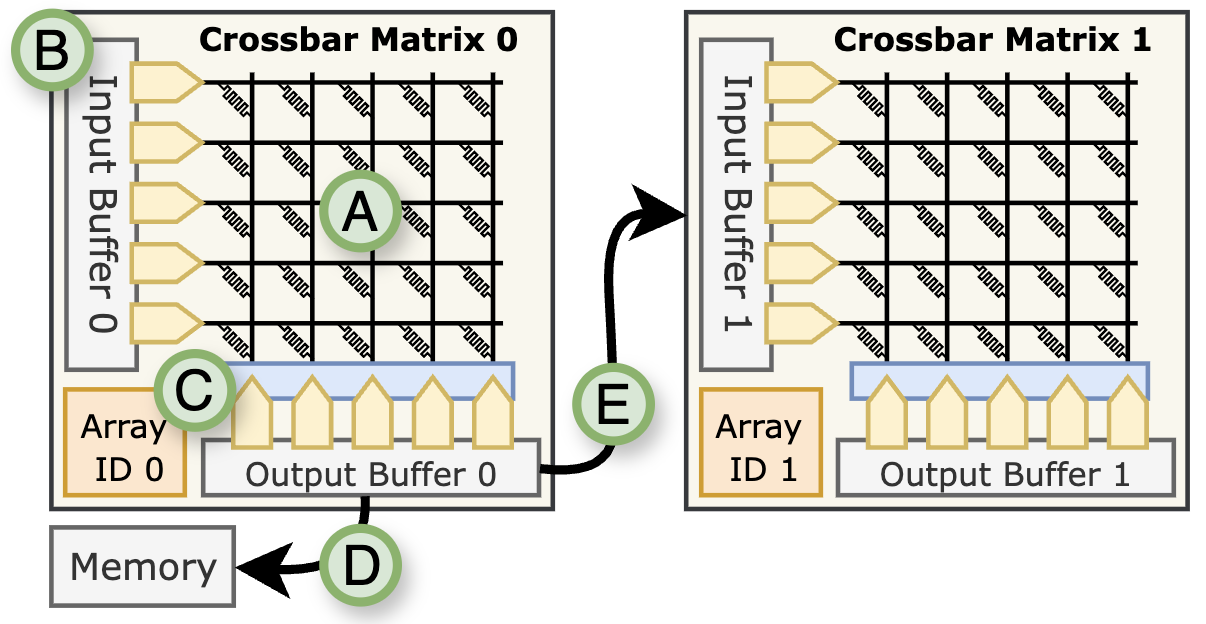
\includegraphics[scale=0.42]{figures/compute_arrays.png}
    \caption{RoCC Commands in action}
    \label{fig:rocc_commands}
\end{figure}

\subsection{Analog Coprocessor}
The analog coprocessor is organized into one or more compute arrays, each serving as an independent processing unit for analog operations.
Every compute array contains three ISA-visible components:
\begin{itemize}
    \item \textbf{Analog array}---contains the programmed analog conductance values. 
        Importantly, in this work we do not optimize the implementation for programming the analog arrays as such work requires substantial device-specific details and for program-once applications is not a major factor in overall system performance.
    \item \textbf{Input buffer}---holds the input operand vector for the MVM operation.
        These values are converted into analog voltages by the array's digital-to-analog converters (DACs).
    \item \textbf{Output buffer}---holds the result of the analog computation as digital values after conversion by analog-to-digital converters (ADCs).
\end{itemize}

For the CPU to coprocessor interface we adopt the conventions of the Rocket Custom Coprocessor (RoCC) interface. \cite{Asanović:EECS-2016-17}
The RoCC interface is an extension point that lets custom coprocessors integrate directly with the CPU pipeline.
Five core instructions form the basis of accelerator and are represented in Figure~\ref{fig:rocc_commands}. 
As noted above, rather than passing individual values in the instructions, we opt to use the local SRAM for passing data between the core and coprocessor.
This is a significant advantage when using multiple arrays per coprocessor.
By allowing each coprocessor to individually perform memory accesses through a dedicated memory port---shared among all arrays within the coprocessor---the RISC-V CPU can perform other operations rather than individually writing operands through the RoCC interface.

This design choice also leads to a uniform structure for the ISA extensions.
Each instruction uses \textit{rs1} to specify the array within the coprocessor, and \textit{rs2} to specify the starting address of the memory access for the given operation.
Finally, since we are focusing on an HPC accelerator, we use a floating point interface for the coprocessors under the assumption that each ISA-visible array is actually multiple arrays using a scheme for combining outputs as in prior work~\cite{8416841,10.1145/3581784.3607077}.
In systems tailored for neural network inference operations, these operations would likely need to be performed on the general purpose CPU rather than in dedicated hardware within the coprocessor.

\begin{figure}[ht]
    \centering
    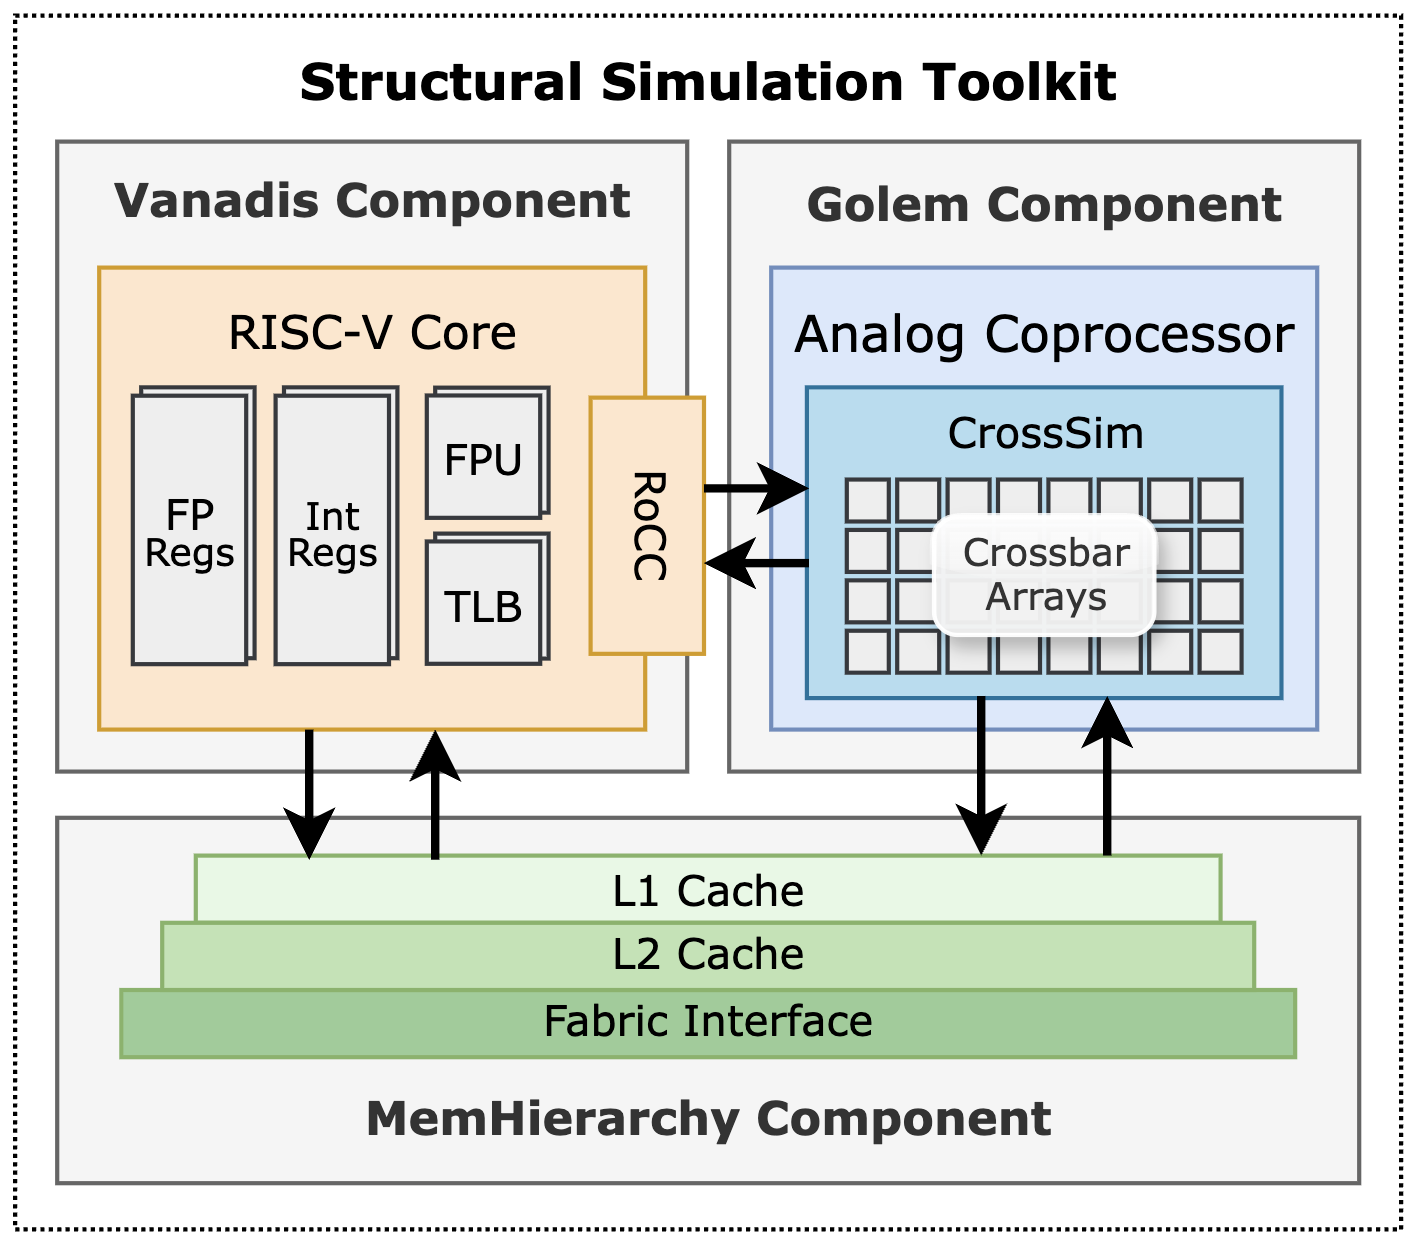
\includegraphics[scale=0.30]{figures/arch_detailed.png}
    \caption{System Architecture showing component integration in SST}
    \label{fig:architecture}
\end{figure}


A typical analog computation begins with the processor configuring a compute array using \textit{mvm.set} (Symbol A in Figure~\ref{fig:rocc_commands}), followed by \textit{mvm.l} (Symbol B) to load the operand vector.
Once both the matrix and vector are staged locally, the \textit{mvm} instruction (Symbol C) initiates computation within the analog array, producing results in the output buffer.
These results can either be stored back to memory with \textit{mvm.s} (Symbol D) or forwarded directly to another array using \textit{mvm.mv} (Symbol E) to enable multiple-stage processing without additional memory traffic.
Cascading MVM operations across multiple arrays within the same tile allows for complex transformations to be executed entirely without off-chip memory accesses, keeping all intermediate data at the source of computation.

% \subsection{Memory Hierarchy}
% The memory hierarchy is designed to sustain high-throughput demands of tiles while preserving full cache coherence across the mesh.
% Each tile's private L1 data and instruction caches have access to the execution pipeline, where operand fetch and result writebacks are issued in parallel. 
% A shared L2 cache connects to the rest of the system through a high-radix mesh router with dedicated ports for each tile.



\subsection{System Simulation Model}
The architecture in Figure~\ref{fig:architecture}, is realized by three specialized SST components: \textit{Vanadis}, \textit{MemHierarchy}, and \textit{Golem} .
\textit{Vanadis} models an out-of-order RISC-V core with configurable reorder buffers, pipeline widths, functional units, and load/store queues.
\textit{MemHierarchy} implements the private L1 and shared L2 caches, a directory-based MESI protocol, and DRAM controllers linked through a high-radix mesh router.
The mesh provides dedicated ports for every core, accelerator, and memory controller enabling multi-core computation. 
\textit{Golem} models the analog accelerator, including crossbars and buffers.
Together, these components enable full-system execution of RISC-V binaries while tracking pipeline behavior, performance and utilization in a HPC-class models.

% The accelerator has DMA 

% Are RoCC instructions blocking/non blocking?
% How does RoCC integrate with vanadis timing model?
% How are DMA requests handled-immediate or queued?

\section{Software Stack}
For software development on the proposed system we have developed an initial software infrastructure to support the development of complex applications.
This software stack builds on the existing RISC-V software infrastructure with modifications to support the proposed accelerator.
Specifically, we modify LLVM 15.0 to emit the RoCC instructions mentioned in the previous section and develop a low-level user library to invoke those functions.
On top of this low-level library we build custom BLAS-like kernels for matrix-vector and matrix-matrix operations, and use OpenMP to distribute tasks across the tiles of the proposed system.  

\begin{figure}[ht]
\centering
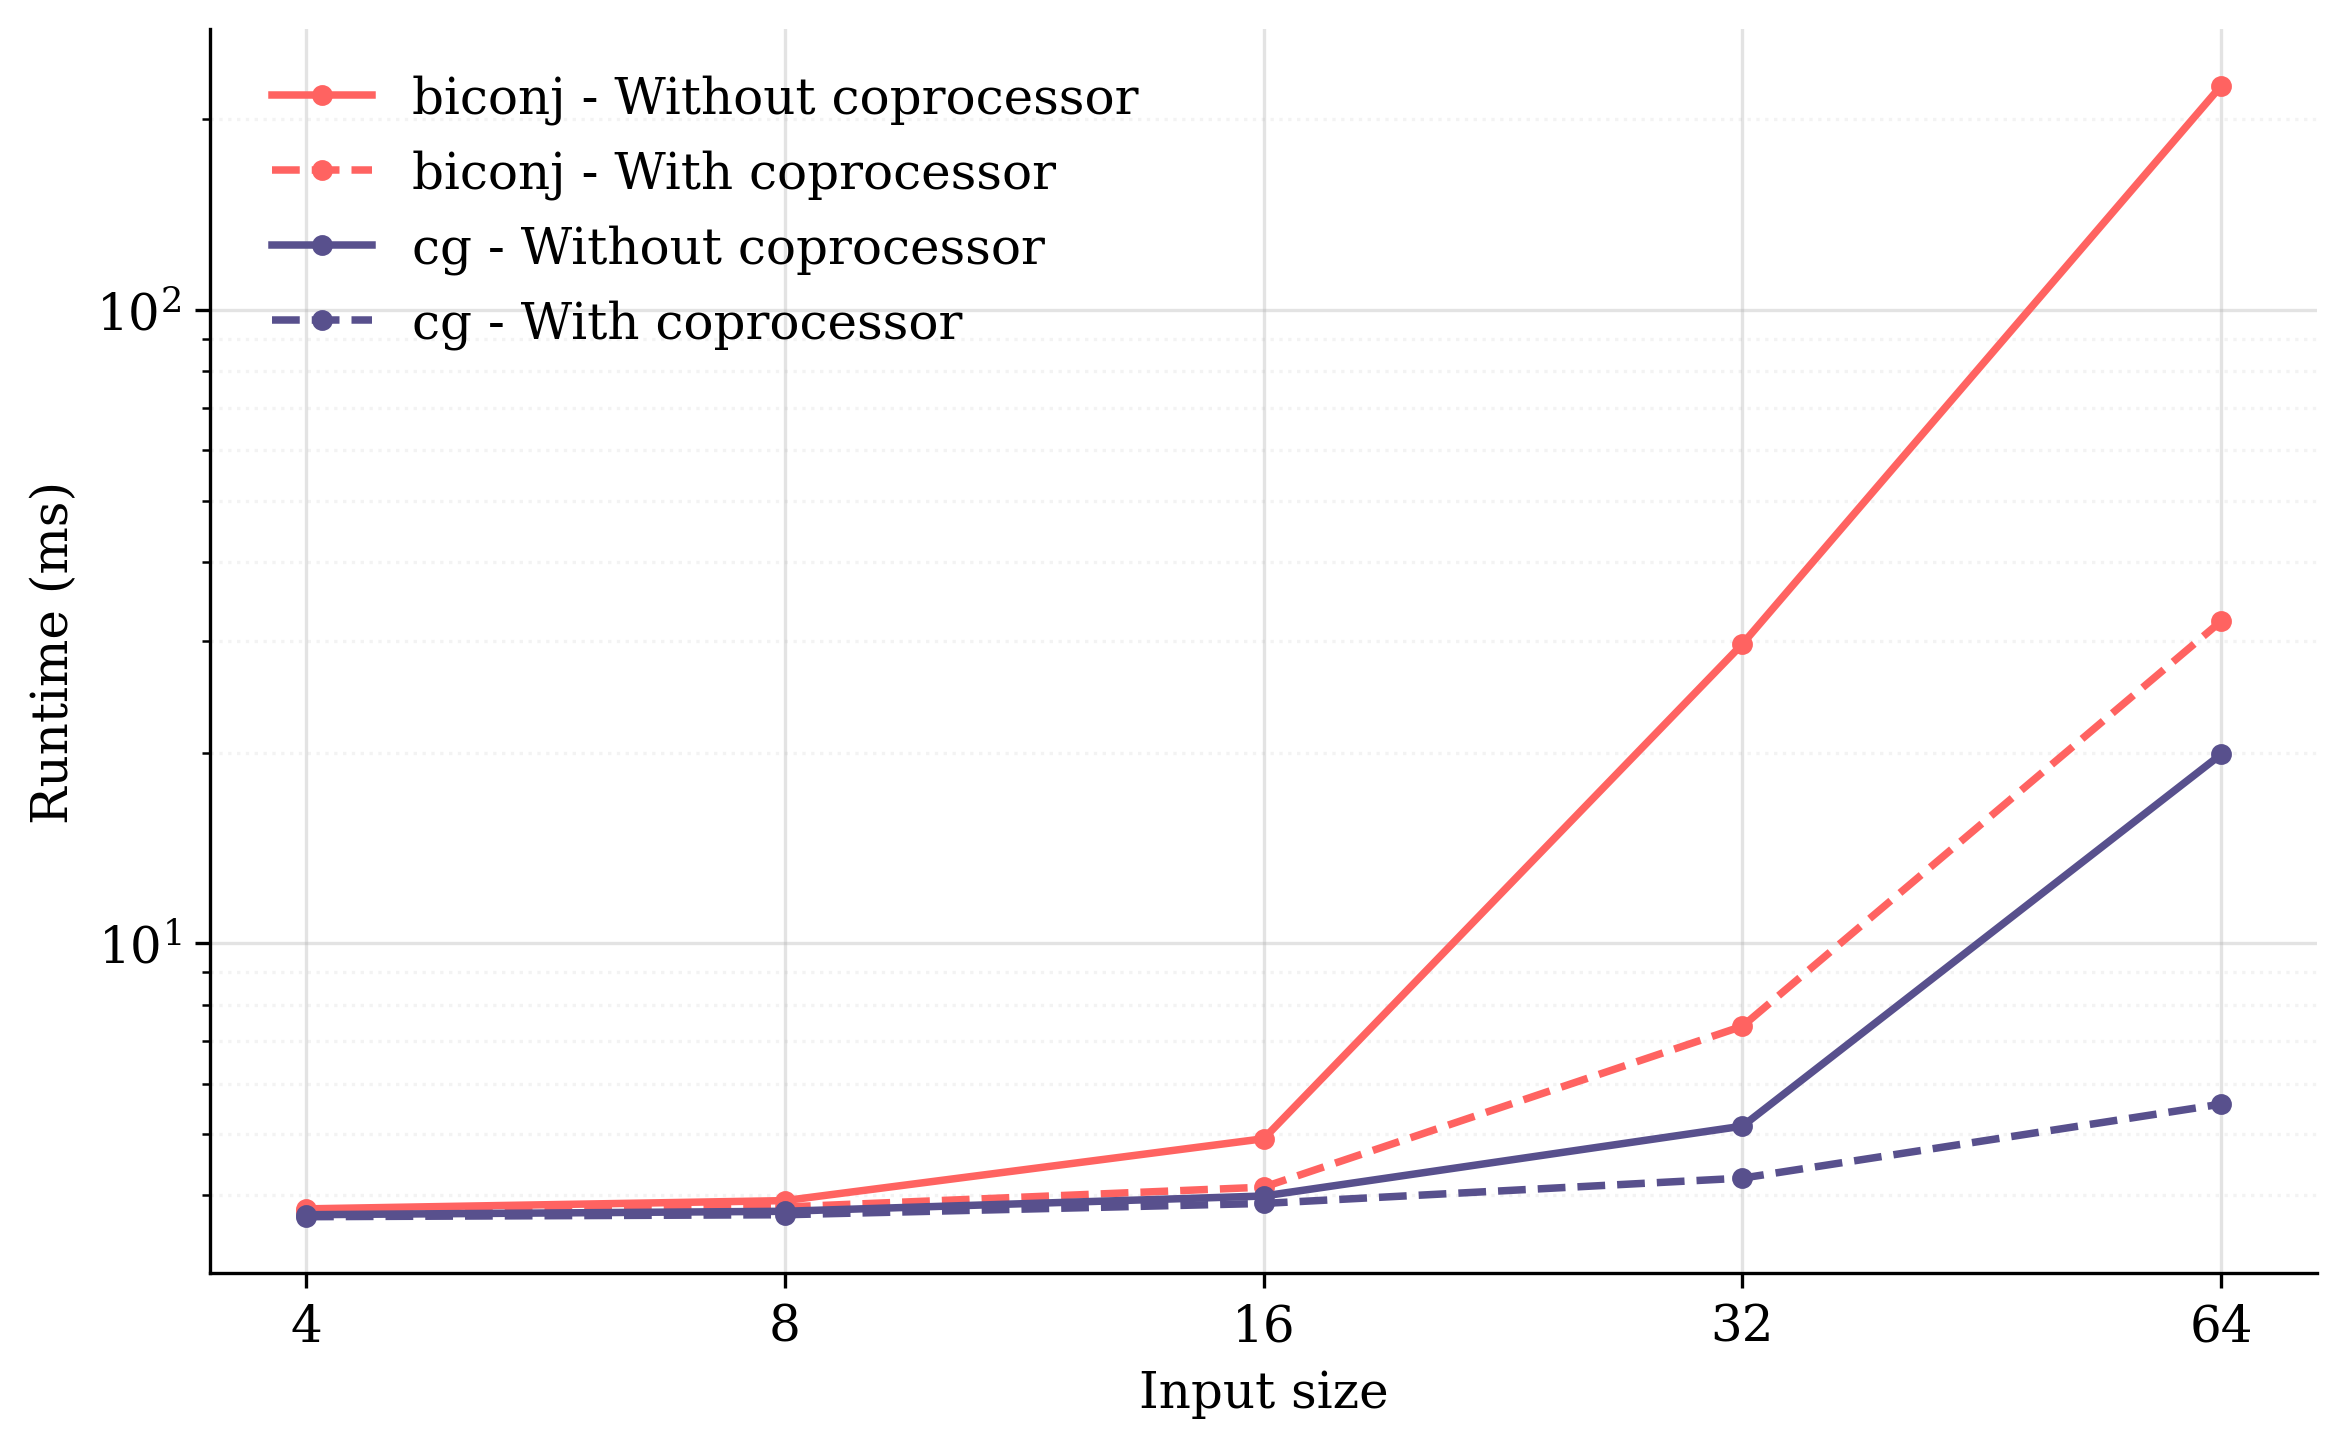
\includegraphics[scale=0.42]{figures/with_without.png}
\vspace{-10pt}
\caption{Runtime Comparison of CG + BiCGStab as N grows}
\vspace{-10pt}
\label{fig:single}
\end{figure}

\subsection{Analog BLAS}
Given the ubiquity of BLAS in HPC applications, we select it as the primary user-facing interface to the analog arrays.
Importantly, we only implement BLAS kernels that can be readily mapped to the proposed analog coprocessor, specifically \texttt{gemm} and \texttt{gemv} in both real and complex variations.
%TODO: Cite to complex expansion if space
In addition to providing a well-known interface, these functions also perform two essential operations for the analog coprocessor, scaling, and size-agnostic mapping.

Analog arrays typically require some form of scaling for optimal performance.
When using a fixed-point interface, values must be scaled into the range of [-1,1] or [0,1] to ensure that the underlying analog ranges are fully used.
With a floating-point interface as evaluated here, scaling is less essential; however, it can take load off of the hardware floating-pointing emulation within the coprocessor.

Unlike digital systems where BLAS functions can take arbitrarily sized matrices, each tile's analog coprocessor has a maximum supported matrix size.
Moreover, matrices and vectors which are not integer multiples of the underlying array size require partitioning and/or zero-padding for mapping to a given array.

To handle both of these operations, the developed AnalogBLAS functions used a specialized \texttt{AnalogMatrix} object to provide an interface for programmed arrays.
Internally AnalogMatrices allocate arrays from a tile coprocessor's pool, track which array identifiers are associated with each matrix, and track scale factors which are used to undo scaling operations providing the programmer with a transparent interface to the BLAS functions.
Importantly, in our current implementation a given tile can only allocate arrays within the tile, support for problems spanning multiple tiles is handled through OpenMP.

\subsection{Multi-tile Operations using OpenMP}

To scale problems beyond a single tile, we use an unmodified RISC-V OpenMP implementation.
Importantly, in the current implementation matrices and inputs are manually partitioned such that each tile's portion of the matrix is at most the maximum matrix capacity of each tile based on the number of analog arrays.
This leads to an interesting insight for analog acceleration for HPC workloads, the use of analog arrays implies that the system must use weak rather than strong scaling.
Although it is possible to reduce the overall portion of the problem allocated to each tile, under-utilizing arrays creates significant inefficiencies which should be avoided.

\begin{figure}[ht]
    \centering
    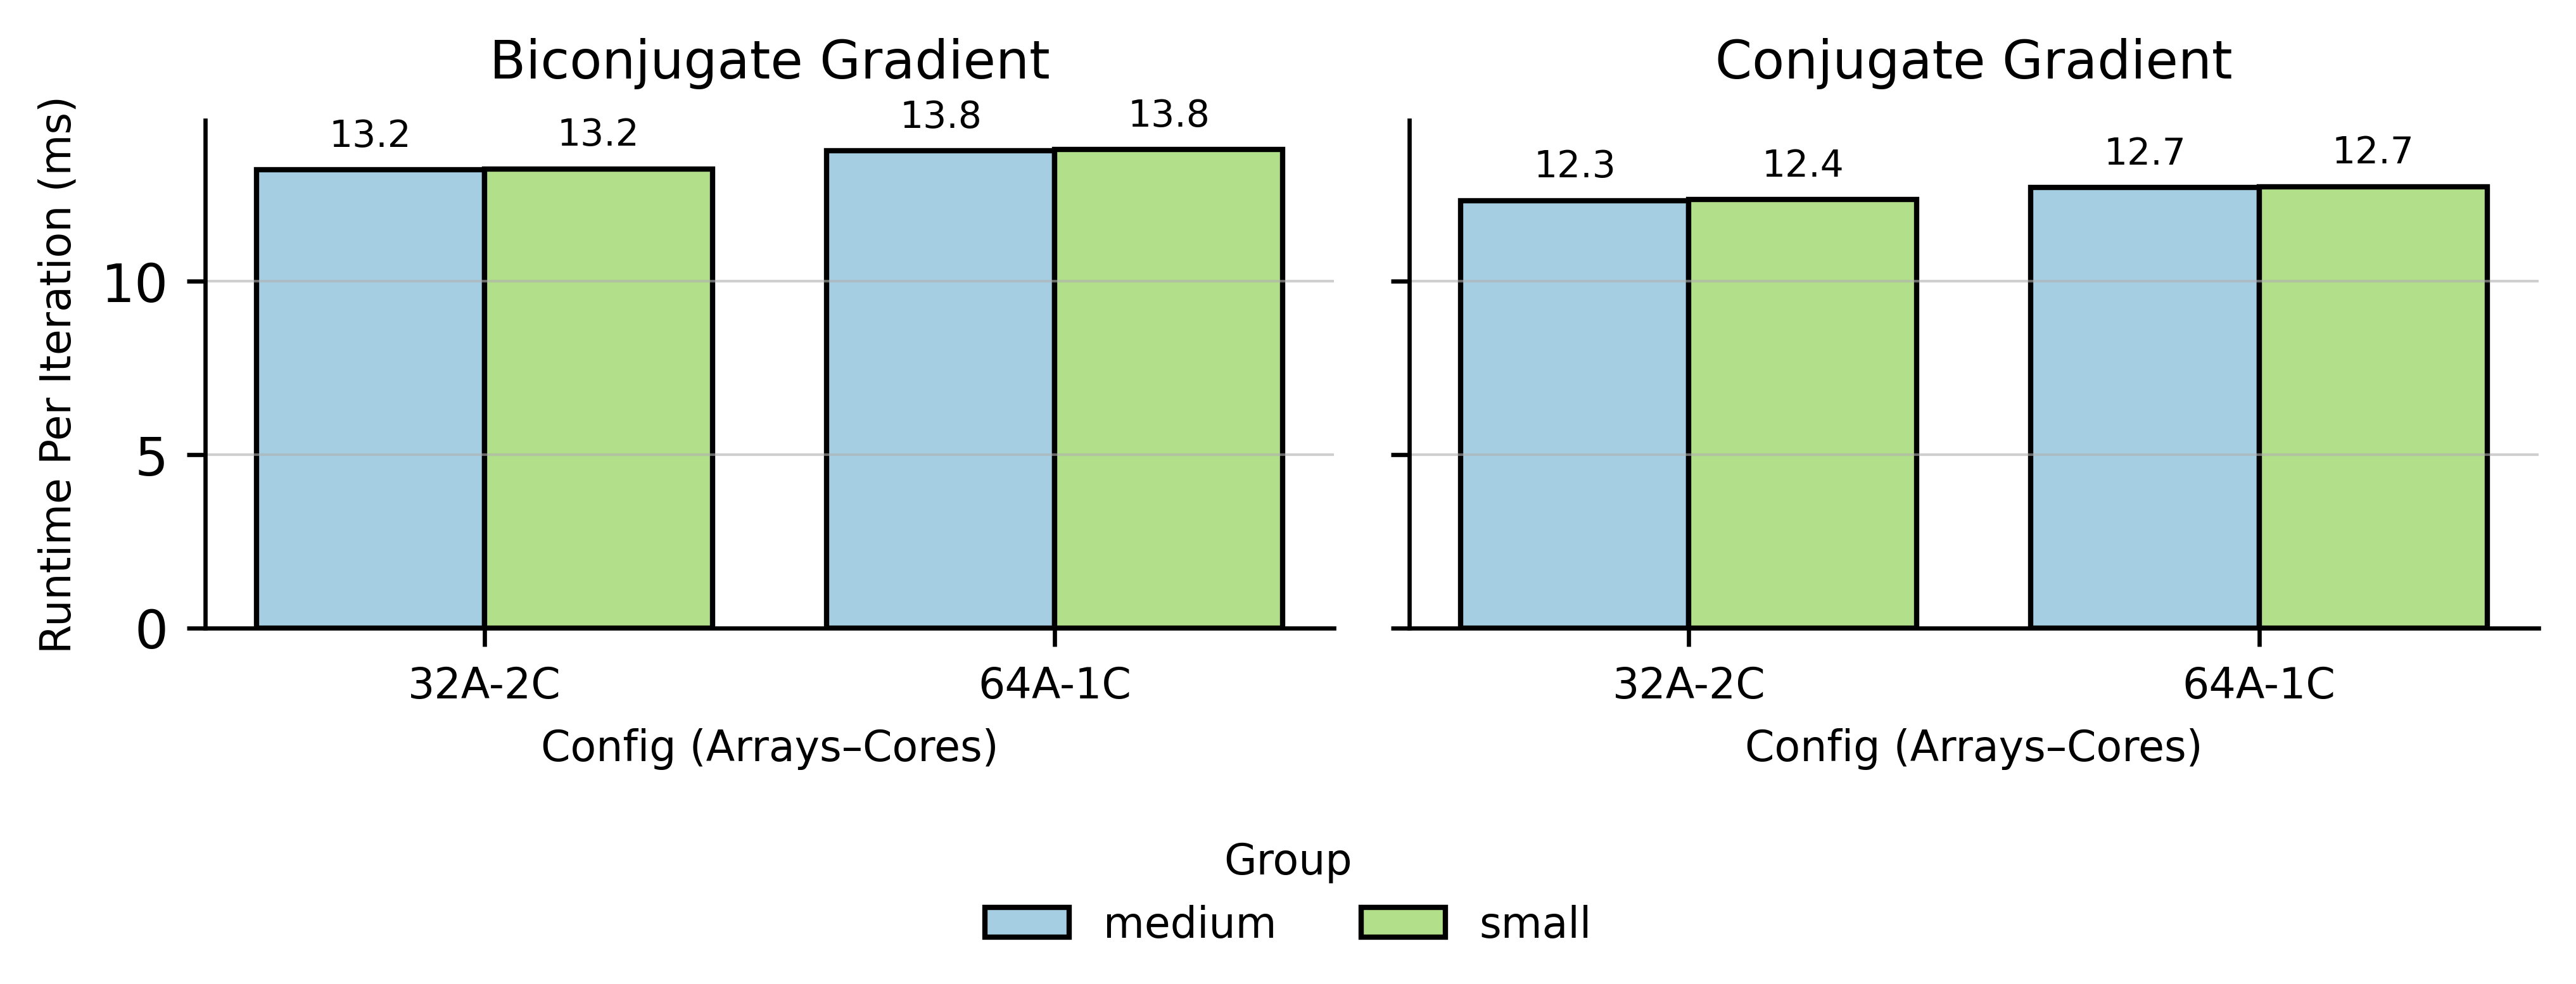
\includegraphics[scale=0.42]{figures/results.png}
    \vspace{-10pt}
    \caption{Runtime Comparison of CG + BiCGStab}
    \label{fig:array_core}
    \vspace{-18pt}
\end{figure}

\subsection{Implementing Iterative Linear Solvers}

Using our Analog BLAS implementation and OpenMP the iterative solvers we implement a pair of iterative linear solvers, Conjugate Gradient CG and BiCG-Stab.
The matrix is partitioned with a two level recursive partitioning, first allocating contiguous blocks to the tiles, and subsequently partitioning those blocks across multiple arrays.
CG and BiCG are the same solvers implemented by Feinberg et al., in prior work~\cite{8416841}; however, by building on the RISC-V software stack we are able to build a more robust and extensible implementation using standard libraries. 


\section{Evaluation}


To evaluate our system architecture, we selected two widely-used iterative linear solvers CG and BiCG-Stab.
Importantly, although iterative linear solvers are typically used for sparse matrices, to focus the analysis in this work we use a pair of synthetic dense matrices.
The convergence of the solvers was verified on smaller test cases such that only 10 iterations were simulated for this larger benchmarking effort.
Additionally, we assume that the floating-point emulation from prior work avoids additional iterations caused be analog imprecision.
Co-simulation of both analog precision and performance is an important topic for future work.

\subsection{Experimental Setup}

Our first experiment measures how the runtime of CG and BiCG-Stab scales with increasing problem size $N$, comparing single core executions with and without a single analog accelerator.
In this analysis the tile has as co-processor array size of $64\times64$ such that only a single array is needed.
This comparison allows us to quantify the accelerator’s contribution to performance and identify the scaling behavior of each solver.
We vary $N$ over a range in multiples of two. 
The results provide insight into how hardware acceleration affects runtime efficiency.


Our second experiment uses a fixed-size $1024\times1024$ dense matrix with $128\times128$ analog MMV arrays. This means a total of 64 arrays are required for the full application, which we consider in two hardware configurations:
\begin{enumerate}
    \item \textbf{Single-tile system} with 64 compute arrays
    \item \textbf{Two-tile system} with 32 compute arrays per tile
\end{enumerate}

Each configuration is tested under two pipeline designs:
\begin{itemize}
    \item \textbf{Small pipeline} --- 32\,KB L1 caches, 256\,KB L2 cache, 2-wide pipeline two floating-point units (FPUs), two integer units (IUs), and a 64-entry reorder buffer (ROB)
    \item \textbf{Large pipeline} --- 32\,KB L1 caches,1\,MB L2 cache, 6-wide pipeline, four FPUs, four IUs, and a 256-entry ROB
\end{itemize}

\subsection{Discussion}


In our first experiment, shown in Figure~\ref{fig:single} , runtimes without the accelerator increase sharply as $N$ approaches 64, whereas accelerator-enabled trials scale far more gracefully.
This single-core, single-accelerator comparison provides evidence that the accelerator delivers  performance gains, underscoring its potential for efficient deployment in HPC workloads.


%  algorithm  input_size  num_arrays    runtime
%4    biconj           4           0    3.80800
%1    biconj           8           0    3.92385
%7    biconj          16           0    4.91428
%5    biconj          32           0   29.69200
%2    biconj          64           0  225.94900

%0    biconj           4           1    3.77589
%6    biconj           8           1    3.83407
%3    biconj          16           1    4.12084
%8    biconj          32           1    7.39816
%9    biconj          64           1   32.27280

%9        cg           4           0    3.72803
%1        cg           8           0    3.77462
%5        cg          16           0    3.99011
%4        cg          32           0    5.14434
%8        cg          64           0   19.88550

%7        cg           4           1    3.70103
%0        cg           8           1    3.72746
%6        cg          16           1    3.88398
%3        cg          32           1    4.25867
%2        cg          64           1    5.57354


Across the architectural and CPU configurations, BiCGStab consistently required longer runtimes than CG.
The marginal performance gap between the small and large pipeline designs informs that \emph{I/O operations—not core or pipeline width—are the dominant bottleneck}, compounded by accelerator communication overhead.
In both solvers, runtime decreased as core count increased, demonstrating that performance scales with parallelism. More investigation must be looked into in this problem space.

\section{Conclusion}

We have presented the first full-system simulation study of a hybrid analog–digital architecture that tightly couples analog matrix–vector multiplication accelerators with general-purpose RISC-V cores.
Using our SST-based simulator, we have demonstrated the potential benefits of analog hardware for HPC applications, and shown how the openness of the RISC-V ISA speeds the development of new hardware by taking advantage of a mature software stack.

Importantly, this work is only the first step in both the development of hybrid analog-digital systems using general purpose RISC-V processors.
There are potential improvements across the entire hardware stack which researchers can explore using the simulation infrastructure presented in this work.
On the hardware side, there are significant potential improvements to both the memory system, replacing our caches with scratchpads, and optimizing these scratchpads for the memory access patterns common for analog accelerators.
Furthermore, since our general-purpose CPU is specifically supporting the analog hardware, vector support using the RISC-V Vector extension would likely improve system throughput.
Additionally, we plan to explore the costs of moving the emulation of floating point operations from a hardened---and by extension inflexible---block within the accelerator to a software implementation running on our general-purpose tile processor.
On the software side, we are exploring further extensions to our analog BLAS library and working on an MLIR-based compiler infrastructure to further simplify the deployment of applications for analog accelerators.
On the algorithm side, we are exploring methods to improve the realism of our algorithms, incorporating preconditioners and extending our work to GMRES and other widely used iterative linear solvers.
Finally, on the simulation side, by coupling these SST simulations with CrossSim, an accuracy simulator for analog arrays, we plan to explore the potential for mixed-precision analog solvers.
Potentially increasing the total number of iterations to convergence while improving overall system performance through more efficient analog mappings.
By building on our extensible simulation framework for hybrid architectures, researchers from numerous domains can make explore important aspects of these analog + RISC-V architectures for HPC and other applications.


% Using an extended \textit{Vanadis} model in SST and a custom analog accelerator element, we evaluated two representative solvers—CG and BiCGStab—across four core–array configurations and pipeline designs.


% Our results show that BiCGStab consistently incurs higher runtime than CG, with only modest sensitivity to pipeline width and functional unit count due to the dominant role of I/O and analog accelerator latency.
% Scaling the number of cores relative to available analog arrays produced measurable reductions in runtime for both solvers.

% This work establishes an open, extensible simulation framework for hybrid architectures, enabling researchers to explore algorithm–architecture co-design without the cost of fabricating hardware.
% Future work will focus on expanding the software toolchain with a C++ library for analog kernel invocation, a dedicated compiler to generate analog-enabled instructions, and MLIR passes to automatically map linear and convolution operations to analog kernels.
% We also plan to extend our evaluation to large-scale, multicore simulations to assess accelerator performance, memory contention, and workload management.



\section*{Acknowledgment}
This article has been authored by an employee of National Technology \& Engineering Solutions of Sandia, LLC under Contract No. DE-NA0003525 with the U.S. Department of Energy (DOE). The employee owns all right, title and interest in and to the article and is solely responsible for its contents. The United States Government retains and the publisher, by accepting the article for publication, acknowledges that the United States Government retains a non-exclusive, paid-up, irrevocable, world-wide license to publish or reproduce the published form of this article or allow others to do so, for United States Government purposes. The DOE will provide public access to these results of federally sponsored research in accordance with the DOE Public Access Plan https://www.energy.gov/downloads/doe-public-access-plan.

\bibliographystyle{ACM-Reference-Format}
\bibliography{ref}

\end{document}
